\documentclass[aspectratio=169]{beamer}
\usepackage[utf8]{inputenc}
%\usepackage[width=160,height=90]{geometry}
\usepackage{graphicx}
\usepackage{multicol}
\usepackage{hyperref}

\renewcommand{\sfdefault}{phv}

\usetheme{Montpellier}

\definecolor{adngreen}{RGB}{51,122,183} %d9534f %337ab7  0,167,127 | 51,122,183 | 235, 83, 79
\setbeamercolor{title}{fg=white}

\setbeamercolor{frametitle}{fg=white}
\setbeamercolor{structure}{bg=adngreen,fg=adngreen}
\setbeamercolor{subsection in sidebar}{fg=white}





\title{\textbf{M183} \\Insecure Direct Object Reference}
\author{Timo Bonomelli, Patrick Günthard}



\AtBeginSection[]
{
  \begin{frame}
    \frametitle{Inhalt}
    \tableofcontents[currentsection]
  \end{frame}
}

\begin{document}

\frame{\titlepage}

%\begin{frame}
%  \frametitle{Table of Contents}
%  \tableofcontents
%\end{frame}
\section{Verwundbarkeit}


\begin{frame}
  \frametitle{What is \textit{Insecure Direct Object References}}
  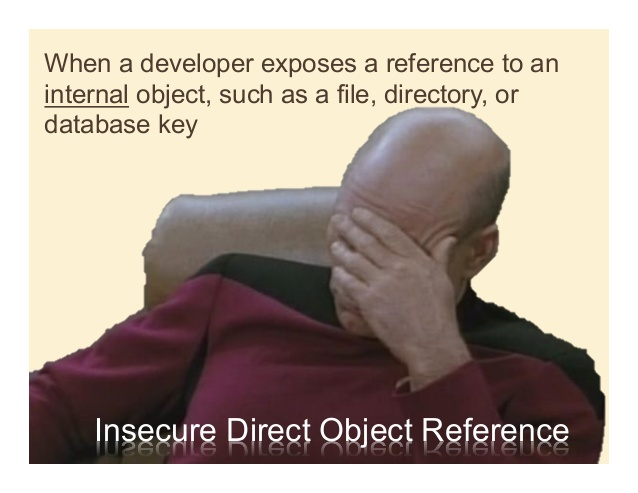
\includegraphics[width=8cm]{meme}
\end{frame}

\subsection{Gefahren}
 
\begin{frame}
  \frametitle{Gefahren}
  \begin{itemize}
  \item \textbf{Von wem geht die Gefahr aus?} Jeder Benutzer welcher nur teilweisen Zugriff auf gewisse Daten hat
  \item \textbf{Angriffsansatz:} Der Angriffer, ein authorisierter System-User, ändert ein parameter welcher direkt mit einem Systemobjekt/Parameter referenziert zu einem anderen Objekt/Parameter, zu dessem Zugriff er nicht berechtigt ist. 
  \item \textbf{Sicherheits-Lücke:} Applilationen überprüfen nicht bei jedem Zugriff die authorisierung
  \end{itemize}
\end{frame}

\subsection{Beispiel}

\begin{frame}[fragile]
  \label{examplecode}
  \frametitle{Example: Code}
  \textit{Beispiel Website:}\\\tiny
\dots
\begin{verbatim}
String query = "SELECT * FROM accts WHERE account = ?";
PreparedStatement pstmt = connection.prepareStatement(query , ... );
pstmt.setString( 1, request.getParameter("acct"));
ResultSet results = pstmt.executeQuery();
\end{verbatim}
\dots\\
\tiny\textit{2010 OWASP - CC-BY-SA}
\normalsize
\end{frame}


\begin{frame}
  \frametitle{Beispiel: Angriff}
  \begin{multicols}{2}
   \LARGE{Normaler Zugriff}\\\normalsize Example URL: \small\texttt{http://example.com/app/ accountInfo?acct=\textit{myacct}}\\
   \normalsize{Resultat:}\\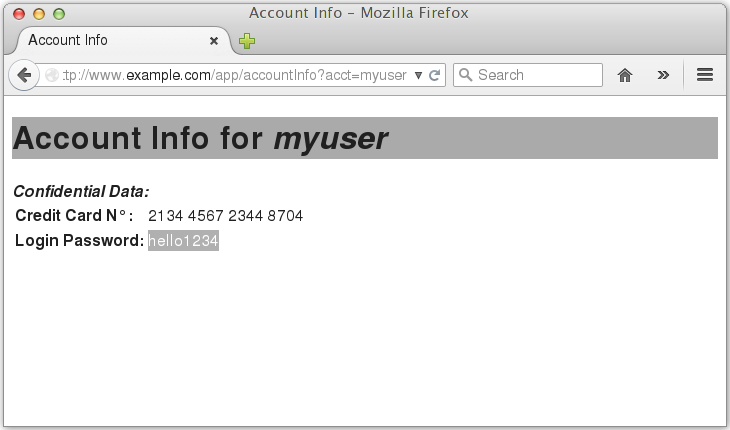
\includegraphics[width=5cm]{example_web_s1}\\
   \LARGE{Angriff}\\\normalsize Example URL: \small\texttt{http://example.com/app/ accountInfo?acct=\textit{notmyacct}}\\
   \normalsize{Resultat:}\\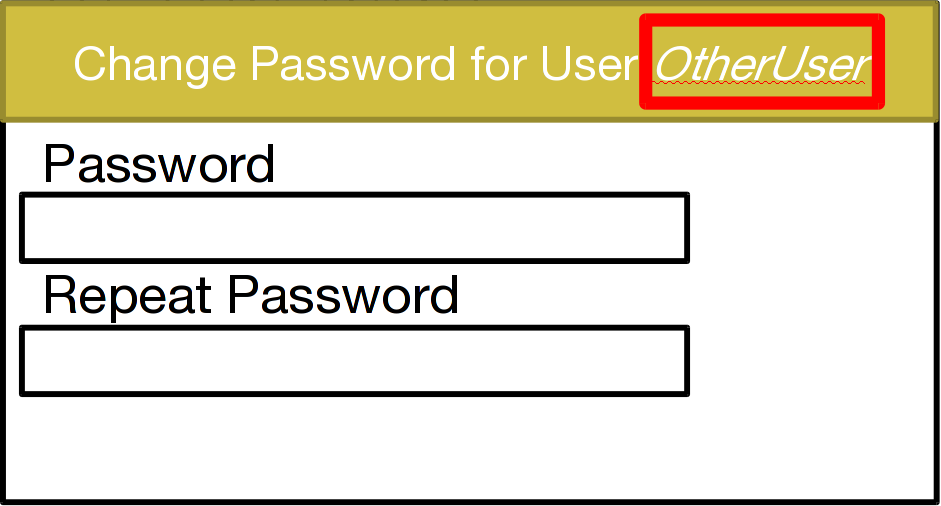
\includegraphics[width=5cm]{example_web_s2}\\
  \end{multicols}
\end{frame}

\begin{frame}
  \frametitle{SQL Injection Attacke (OWASP A1)}
  URL:\\ \texttt{app/accountInfo?acct=\textit{myacct'; DROP accts; }} (\ref{examplecode})
\end{frame}


\section{Wie kann man sich vor Angriffen schützen?}

\subsection{Session Basiert}

\begin{frame}
  \frametitle{Session}
  \begin{itemize}
  \item Keine \textit{Direct Object Reference} müssen an den client gesendet werden, sie können auf dem Server in der Session gespeichert werden.
  \item Wenn trotzdem Refernzen benötigt werden, können sie sich von den ursprünglichen daten unterscheiden und gemappt werden.
  \end{itemize}
\end{frame}

\subsection{Check Authorization on every access}

\begin{frame}
  \frametitle{Authorization}
  \begin{itemize}
    \item Every access is checked if the user is authorized to do that. Example: A random token can be created for each user which then is checked every time the user accesses the page
  \end{itemize}
\end{frame}

\subsection{Solutions and Problems}

\begin{frame}
  \frametitle{Solutions and Problems}
\tiny
  \begin{tabular}{|l|p{4cm}|p{4cm}|}
    \hline
    & \textbf{Advantage} & \textbf{Disadvantage} \\\hline
    \textbf{Session Based} & Only one authorization has to be done, access data for Database etc. is saved on the server and is not accessible by the attacker & A session uses a lot of memory for each user. For applications with a high number of users, a session for each client is not possible i.e. a non-session solution has to be implemented \\\hline
    \textbf{Authorization} & No Session is needed i.e. less memory is used and more users can access the application & Authorization is needed every time the user accesses data which is more complex to implement\\\hline
  \end{tabular}
\end{frame}


\section{Summary}

\begin{frame}
  \frametitle{Summary}
  \begin{itemize}
    \item Serious Issue
    \item Easily preventable
    \item Several fixing solutions
  \end{itemize}
\end{frame}

\begin{frame}
  \frametitle{End}
  Sources:\\
  \begin{itemize}
    \item \href{https://www.owasp.org/index.php/Top_10_2010-A4-Insecure_Direct_Object_References}{OWASP: 2010-A4-Insecure Direct Object References}
    \item \href{https://en.wikipedia.org/wiki/HDIV}{Wikipedia: HDIV}
  \end{itemize}


\includegraphics[width=1cm]{cc.png}
  
\end{frame}

\end{document}